\documentclass{standalone}
\usepackage[utf8]{inputenc}
\usepackage{tikz}

\usetikzlibrary{positioning}

\tikzstyle{inputNode}=[draw,circle,minimum size=10pt,inner sep=0pt]
\tikzstyle{stateTransition}=[-stealth, thick]

\begin{document}
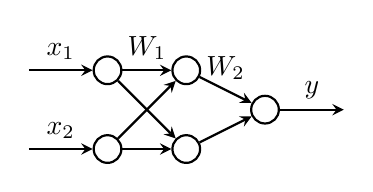
\begin{tikzpicture}
	\node[inputNode, thick] (i1) at (6, 0.5) {};
	\node[inputNode, thick] (i2) at (6, -0.5) {};

	\node[inputNode, thick] (h1) at (7, 0.5) {};
	\node[inputNode, thick] (h2) at (7, -0.5) {};

	\node[inputNode, thick] (o1) at (8, 0) {};

	\draw[stateTransition] (5, 0.5) -- node[above] {$x_1$} (i1);
	\draw[stateTransition] (5, -0.5) -- node[above] {$x_2$} (i2);

	\draw[stateTransition] (i1) -- (h1) node[pos=0.5,above] {$W_1$};
	\draw[stateTransition] (i1) -- (h2);
	\draw[stateTransition] (i2) -- (h1);
	\draw[stateTransition] (i2) -- (h2);

	\draw[stateTransition] (h1) -- (o1) node[pos=0.5,above] {$W_2$};;
	\draw[stateTransition] (h2) -- (o1);

	\draw[stateTransition] (o1) -- node[above] {$y$} (9, 0);
\end{tikzpicture}
\end{document}
